\documentclass{article}
\usepackage[utf8]{inputenc}
\usepackage{amsmath}
\usepackage{amsfonts}
\usepackage{tikz}
\usepackage{caption}
\usepackage{adjustbox}
\usetikzlibrary{arrows}

\begin{document}

\section{Maximum degree of $3\Delta_{avg} + 8$}

Maciek: Intro to the algorithm, comparison with DISC algorithm.
(high degree nodes participate as helpers, H-H edges are replaced, low degree nodes are $n/4$ of all nodes)

\subsection{Algorithm}


The algorithm arbitrarily assigns a node to \emph{help} each edge in the demand graph.
While doing so, it ensures that each node helps at most $\beta = \lceil\Delta_{avg}/2\rceil$ edges.


To construct the network, we first construct an \emph{auxiliary graph} $G'$ that is initially equal to the demand distribution graph $G_D$.
Then, we construct the network $N$ from $G'$.

Now we construct the auxiliary graph $G'$ based upon the helper nodes assignment.
If the helping node $k$ is chosen as either $i$ or $j$, then do not modify any edges of $G'$.
Otherwise, if the algorithm helps $k \neq i,j$ to help the edge $(i, j)$, we replace the edge $(i, j)$ in $G'$ with 
2-hop paths through $k$:
$$ p(i,j) = 0$$
$$ p(i,k) = p(i,k) + p(i,j)$$
$$ p(k,j) = p(k,j) + p(i,j)$$
We say that the edges $(i,k)$ and $(k,j)$ added to (and from) intermediate nodes are \emph{intermediate edges}.

Next, we construct the network $N$ based upon the auxiliary graph $G'$.
We start with an empty network $N$.
In $G'$, a node $i$ has two types of new neighbors: 
the set $G_i$ of intermediate nodes that replaced an initial edges of $i$, and the set $H_i$ of nodes in whose edges $i$ is helping.
Among $G_i$ we distinguish the set $G_i^-$ (resp. $G_i^+$) of nodes that are connected with $i$ with an ingoing (resp. outgoing) edges.
For each node $i$, the algorithm constructs two Mehlhorn trees in $N$, one for $G_i^-$ and another for $G_i^+$, and connects its roots to $i$.
(reference to Figure of i,j and helper k)

Note that we skip the set $H_i$ while building the Mehlhorn trees of neighbors of $i$.
However, the connection (possibly indirect) between $i$ and a node $j \in H_i$ appears while building the Mehlhorn tree of $j$.

\medskip

Now we claim that the algorithm has a sufficient number of nodes available as helpers 
 (i.e., the total number of available helpers $n \cdot \beta$ is sufficient to help all $m$ edges).

  $$n \cdot \beta = \frac{n\Delta_{avg}}{2} = m$$

and we conclude that the algorithm is well-defined.

\medskip
\newpage
Now, we upper-bound the maximal final degree of the nodes.
A node $i$ is involved in one Mehlhorn tree
for each node it helped, in total at most $2\beta$ trees.
Furthermore, the node $i$ is connected with one edge to Mehlhorn trees $G_i^+$ and $G_i^-$.
Note that the node $i$ is not involved in the Mehlhorn trees of the intermediate nodes
that replaced a node between $i$ and another node.
%The degree of each node may increase beyond its initial degree because it helps other nodes, and, more importantly, because it may participate in Mehlhorn trees of its neighbors.
A~participation in each Mehlhorn tree adds at most $3$ edges to a node, thus its final degree $\gamma_i$ is

$$\gamma_i \leq 6\beta + 2 \leq 6 \left(\frac{\Delta_{avg}}{2}+1\right) + 2 =  3\Delta_{avg} + 8.$$
%
We conclude that the algorithm produces a network
with maximum degree of $3\Delta_{avg} + 8$.

Remarks.
When a node is assigned to help one of its incident edges, it is the most efficient.
However, the analysis holds for arbitrary assignments.

Now we claim that EPL are within the constant in comparison to optimum.
This is a consequence of near-optimality of Mehlhorn trees.

\section{Dealing with congestion}

Above algorithm has asymptotically optimal congestion.
The lower bound from INFOCOM paper, let's say it's $c$ on the most loaded edge of EgoTree.
Then, our most congested edge is the one connecting the root to the Mehlhorn tree, and it has congestion $c \cdot \Delta_{avg}$.

Introduce p-EgoTree and the new way of constructing them (instead of solving the scheduling, we simulate solving it, and then pack some trees together).
Show its properties: it approximates congestion.

Now we show how to trade the congestion to the increased $\Delta_{max}$.
Using $p$-EgoTrees gives us the $\Delta_{max} = 3\cdot \Delta_{avg} + 6 ) 2 \cdot p \cdot \Delta_{avg}$.
The congestion is then $4/3$ of LPTF, multiplied by $\Delta_{max} / (p \cdot \Delta_{avg})$.
The final congestion bound is due to the number of times the node can help, $\beta_i$.

\newpage

\subsection{Example}

\begin{figure}[!htb]\centering
\begin{minipage}[b]{.3\linewidth}
  \begin{adjustbox}{width=\linewidth}
      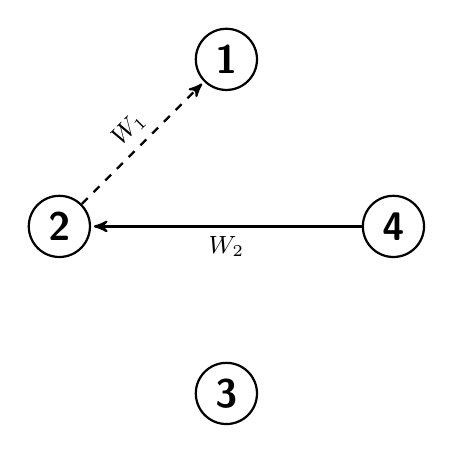
\begin{tikzpicture}[->,>=stealth',shorten >=1pt,auto,node distance=3cm,
          thick,main node/.style={circle,draw,font=\sffamily\Large\bfseries}]

        \node[main node] (1) {1};
        \node[main node] (2) [below left of=1] {2};
        \node[main node] (3) [below right of=2] {3};
        \node[main node] (4) [below right of=1] {4};

        \path[every node/.style={font=\sffamily\small}]
        (2) edge[dashed] node [above,rotate=45] {$W_1$} (1)
        (4) edge node [below] {$W_2$} (2);
      \end{tikzpicture}
  \end{adjustbox}
  \caption*{Demand graph $G_D$}
\end{minipage}
\hspace{0.2 cm}
\begin{minipage}[b]{.3\linewidth}
  \begin{adjustbox}{width=\linewidth}
    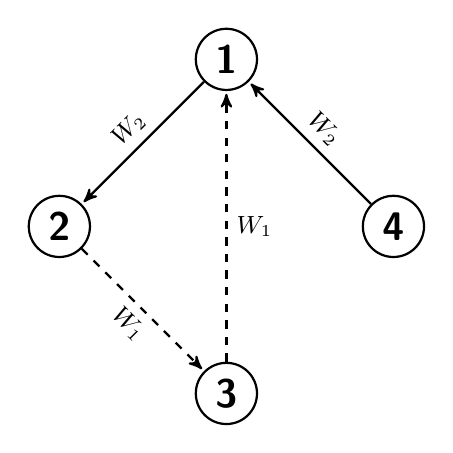
\begin{tikzpicture}[->,>=stealth',shorten >=1pt,auto,node distance=3cm,
      thick,main node/.style={circle,draw,font=\sffamily\Large\bfseries}]

    \node[main node] (1) {1};
    \node[main node] (2) [below left of=1] {2};
    \node[main node] (3) [below right of=2] {3};
    \node[main node] (4) [below right of=1] {4};

    \path[every node/.style={font=\sffamily\small}]
    (1) edge node [above,rotate=45] {$W_2$} (2)
    (2) edge[dashed] node [below,rotate=-45] {$W_1$} (3)
    (3) edge[dashed] node [right] {$W_1$} (1)
    (4) edge node [above,rotate=-45] {$W_2$} (1);
    \end{tikzpicture}
  \end{adjustbox}
  \caption*{Intermediate graph $G'$}
\end{minipage}
\hspace{0.2 cm}
\begin{minipage}[b]{.3\linewidth}
  \begin{adjustbox}{width=\linewidth}
    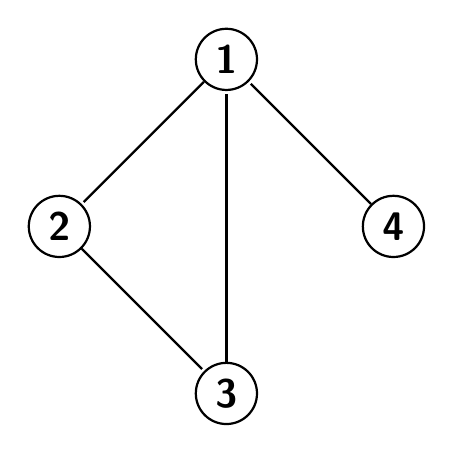
\begin{tikzpicture}[-,>=stealth',shorten >=1pt,auto,node distance=3cm,
      thick,main node/.style={circle,draw,font=\sffamily\Large\bfseries}]

    \node[main node] (1) {1};
    \node[main node] (2) [below left of=1] {2};
    \node[main node] (3) [below right of=2] {3};
    \node[main node] (4) [below right of=1] {4};

    \path[every node/.style={font=\sffamily\small}]
    (1) edge node {} (2)
    (2) edge node {} (3)
    (3) edge node {} (1)
    (4) edge node {} (1);
    \end{tikzpicture}
  \end{adjustbox}
  \caption*{Bounded network $N$}
\end{minipage}
\caption{Running the algorithm on a simple example}
\end{figure}

In this example, $\Delta_{avg} = 1$ thus the limit of the number of times a node can help
is $\lceil\Delta_{avg}/2\rceil = 1$. 
Nodes $1$ and $3$ help the edges $(4,2)$ and $(2,1)$, respectively.
For each node $i$, a Mehlhorn tree is built on the set of nodes that
helped an edge connected to $i$.
The initial degree of $3$ is $0$, thus there is no Mehlhorn tree from it.
The nodes $1$ and $3$ help the only edge of $4$ and $1$, respectively.
The built Mehlhorn trees are simple edges.
Finally, $2$ is connected to an outgoing and an ingoing edge, thus two
Mehlhorn trees including the nodes $1$ and $3$, will be built from $2$.

\newpage

\subsection{Explanatory scheme}

\begin{figure}[!htb]\centering
  \begin{minipage}[b]{.45\linewidth}
    \begin{adjustbox}{width=\linewidth}
      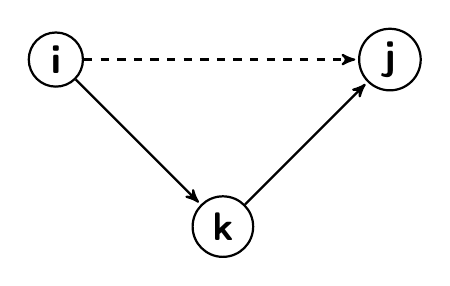
\begin{tikzpicture}[->,>=stealth',shorten >=1pt,auto,node distance=3cm,
        thick,main node/.style={circle,draw,font=\sffamily\Large\bfseries}]

      \node[main node] (1) {k};
      \node[main node] (2) [above left of=1] {i};
      \node[main node] (3) [above right of=1] {j};

      \path[every node/.style={font=\sffamily\small}]
      (2) edge node {} (1)
      (2) edge[dashed] node {} (3)
      (1) edge node {} (3);
      \end{tikzpicture}
    \end{adjustbox}
  \end{minipage}
\end{figure}

\end{document}